% D4 - The merge boundary.
%
% Small, but it is the visual proof that Lambda's advertised weakness - "reconciling
% data between two systems" - was solved rather than described. The rule is half-open
% intervals, so the watermark DATE belongs to exactly one side: the batch side.
\documentclass[border=8pt]{standalone}
% Shared styling for every report diagram.
%
% One colour convention across all four, stated in the legend on D2:
%   BLUE   speed path    - the approximate, low-latency half
%   GREEN  batch path    - the exact, recomputed half
%   GREY   infrastructure- stores and brokers that belong to neither path
%   ORANGE serving       - where the two are reconciled
%
% TikZ rather than draw.io: the report is LaTeX, so these compile as vector art with
% no external asset pipeline, the source is version-controlled beside the code, and
% fonts match the body text exactly. A diagram that can be regenerated from source is
% also a diagram that cannot silently drift from the system it describes.

\usepackage{tikz}
\usepackage{xcolor}
\usetikzlibrary{positioning,arrows.meta,fit,backgrounds,calc,shapes.geometric}

\definecolor{speedblue}{HTML}{1F6FB2}
\definecolor{speedbg}{HTML}{E3F0FA}
\definecolor{batchgreen}{HTML}{2E7D4A}
\definecolor{batchbg}{HTML}{E4F3E8}
\definecolor{servorange}{HTML}{C2660A}
\definecolor{servbg}{HTML}{FCEDDD}
\definecolor{infragrey}{HTML}{5A6672}
\definecolor{infrabg}{HTML}{ECEFF1}
\definecolor{edgegrey}{HTML}{444C54}

\tikzset{
  box/.style={
    draw, rounded corners=2pt, align=center, inner sep=5pt,
    font=\scriptsize, minimum height=8mm, line width=0.5pt,
  },
  speed/.style ={box, draw=speedblue,  fill=speedbg,  text=black},
  batch/.style ={box, draw=batchgreen, fill=batchbg,  text=black},
  serv/.style  ={box, draw=servorange, fill=servbg,   text=black},
  infra/.style ={box, draw=infragrey,  fill=infrabg,  text=black},
  ext/.style   ={box, draw=edgegrey, fill=white, dashed, text=black},
  flow/.style  ={-{Stealth[length=4pt]}, draw=edgegrey, line width=0.5pt},
  speedflow/.style={flow, draw=speedblue},
  batchflow/.style={flow, draw=batchgreen},
  lbl/.style   ={font=\tiny\itshape, text=edgegrey, inner sep=1.5pt},
  zone/.style  ={draw=edgegrey, dashed, rounded corners=3pt, line width=0.4pt,
                 inner sep=7pt},
  % fill=white matters: these labels sit ON the dashed zone border, and without
  % an opaque background the border line runs straight through the text and
  % reads as a strike-through.
  ztitle/.style={font=\scriptsize\bfseries, text=edgegrey, fill=white,
                 inner xsep=3pt, inner ysep=1pt},
}

\begin{document}
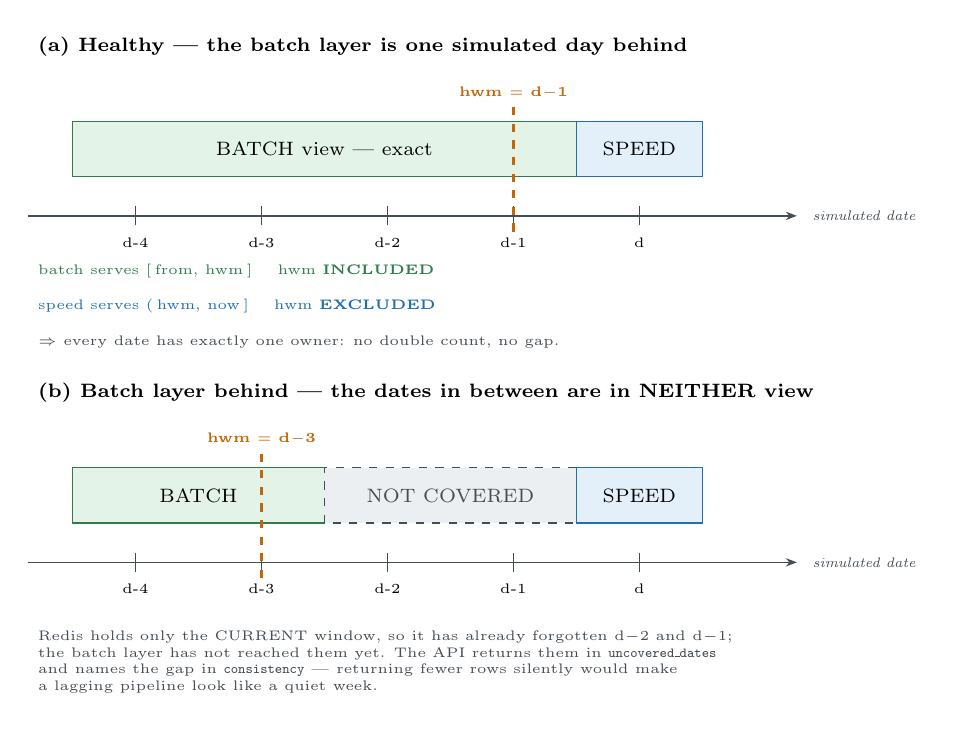
\begin{tikzpicture}[x=16mm, y=10mm]

\newcommand{\daxis}[1]{%
  \draw[flow, draw=edgegrey] (-0.35,#1) -- (5.75,#1);
  \foreach \x/\d in {0/{d-4}, 1/{d-3}, 2/{d-2}, 3/{d-1}, 4/{d}} {
    \draw[edgegrey] (\x+0.5,#1-0.12) -- (\x+0.5,#1+0.12);
    \node[font=\tiny, below=1pt] at (\x+0.5,#1-0.12) {\d};
  }
  \node[font=\tiny\itshape, text=edgegrey, anchor=west] at (5.8,#1) {simulated date};
}

% ============================================ case 1: healthy, one day behind
\node[font=\scriptsize\bfseries, anchor=west] at (-0.35,4.95)
  {(a) Healthy \textemdash\ the batch layer is one simulated day behind};

\fill[batchbg, draw=batchgreen] (0,3.3) rectangle (4,4.0);
\fill[speedbg, draw=speedblue]  (4,3.3) rectangle (5,4.0);
\node[font=\scriptsize] at (2,3.65)   {BATCH view \textemdash\ exact};
\node[font=\scriptsize] at (4.5,3.65) {SPEED};

\daxis{2.8}

% The watermark is a DATE, not the gap between two dates, so it is marked on d-1.
\draw[servorange, line width=1pt, dashed] (3.5,2.6) -- (3.5,4.25);
\node[font=\tiny\bfseries, text=servorange, anchor=south, fill=white, inner sep=1pt]
  at (3.5,4.25) {hwm $=$ d$-$1};

\node[font=\tiny, anchor=west, text=batchgreen] at (-0.35,2.1)
  {batch serves $[\,$from,\ hwm$\,]$ \quad hwm \textbf{INCLUDED}};
\node[font=\tiny, anchor=west, text=speedblue] at (-0.35,1.65)
  {speed serves $(\,$hwm,\ now$\,]$ \quad hwm \textbf{EXCLUDED}};
\node[font=\tiny, anchor=west, text=edgegrey] at (-0.35,1.2)
  {$\Rightarrow$ every date has exactly one owner: no double count, no gap.};

% ============================================ case 2: batch behind, real gap
\node[font=\scriptsize\bfseries, anchor=west] at (-0.35,0.55)
  {(b) Batch layer behind \textemdash\ the dates in between are in NEITHER view};

\fill[batchbg, draw=batchgreen] (0,-1.1) rectangle (2,-0.4);
\fill[infrabg, draw=edgegrey, dashed] (2,-1.1) rectangle (4,-0.4);
\fill[speedbg, draw=speedblue] (4,-1.1) rectangle (5,-0.4);
\node[font=\scriptsize] at (1,-0.75) {BATCH};
\node[font=\scriptsize, text=edgegrey] at (3,-0.75) {NOT COVERED};
\node[font=\scriptsize] at (4.5,-0.75) {SPEED};

\daxis{-1.6}

\draw[servorange, line width=1pt, dashed] (1.5,-1.8) -- (1.5,-0.15);
\node[font=\tiny\bfseries, text=servorange, anchor=south, fill=white, inner sep=1pt]
  at (1.5,-0.15) {hwm $=$ d$-$3};

\node[font=\tiny, anchor=north west, text=edgegrey, align=left] at (-0.35,-2.35)
  {Redis holds only the CURRENT window, so it has already forgotten
   d$-$2 and d$-$1;\\
   the batch layer has not reached them yet. The API returns them in
   \texttt{uncovered\_dates}\\
   and names the gap in \texttt{consistency} \textemdash\ returning fewer rows silently
   would make\\
   a lagging pipeline look like a quiet week.};

\end{tikzpicture}
\end{document}
